%%%%%%%%%%%%%%%%%%%%%%%%%%%%%%%%%%%%%%%%%%%%%%%%%%%%%%%%%%%%%%%%%%%%%%%%%%%%%%%%%%
\begin{frame}[fragile]\frametitle{}
\begin{center}
{\Large Data Exploration  - US Flights}

{\tiny (Ref: mlcourse.ai Assignment 2 – Open Machine Learning Course) }

\end{center}

\end{frame}


%%%%%%%%%%%%%%%%%%%%%%%%%%%%%%%%%%%%%%%%%%%%%%%%%%%%%%%%%%
\begin{frame}[fragile]\frametitle{Problem Info}	
\begin{itemize}
\item Download data from http://stat-computing.org/dataexpo/2009/2008.csv.bz2 
\item (Archived \~ 114 Mb, unzipped - \~ 690 Mb). No need to unzip - pandas can unbzip on the fly.
\item Column Description is at http://www.transtats.bts.gov/Fields.asp?Table\_ID=236
\end{itemize}
\end{frame}

%%%%%%%%%%%%%%%%%%%%%%%%%%%%%%%%%%%%%%%%%%%%%%%%%%%%%%%%%%
\begin{frame}[fragile]\frametitle{Import Libraries}	
\begin{lstlisting}
import numpy as np
import pandas as pd
# pip install seaborn 
import seaborn as sns
import matplotlib.pyplot as plt
\end{lstlisting}
\end{frame}


%%%%%%%%%%%%%%%%%%%%%%%%%%%%%%%%%%%%%%%%%%%%%%%%%%%%%%%%%%
\begin{frame}[fragile]\frametitle{Read Data}	
We load only limited columns
\begin{lstlisting}
dtype = {'DayOfWeek': np.uint8, 'DayofMonth': np.uint8, 'Month': np.uint8 , 'Cancelled': np.uint8, 
         'Year': np.uint16, 'FlightNum': np.uint16 , 'Distance': np.uint16, 
         'UniqueCarrier': str, 'CancellationCode': str, 'Origin': str, 'Dest': str,
         'ArrDelay': np.float16, 'DepDelay': np.float16, 'CarrierDelay': np.float16,
         'WeatherDelay': np.float16, 'NASDelay': np.float16, 'SecurityDelay': np.float16,
         'LateAircraftDelay': np.float16, 'DepTime': np.float16}
		 
path = 'data/2008.csv.bz2'
flights_df = pd.read_csv(path, usecols=dtype.keys(), dtype=dtype)		 
\end{lstlisting}
\end{frame}

%%%%%%%%%%%%%%%%%%%%%%%%%%%%%%%%%%%%%%%%%%%%%%%%%%%%%%%%%%
\begin{frame}[fragile]\frametitle{Describe Data}	
Check the number of rows and columns and print column names.
\begin{lstlisting}
print(flights_df.shape)
print(flights_df.columns)
>>
(7009728, 19)
Index(['Year', 'Month', 'DayofMonth', 'DayOfWeek', 'DepTime', 'UniqueCarrier',
       'FlightNum', 'ArrDelay', 'DepDelay', 'Origin', 'Dest', 'Distance',
       'Cancelled', 'CancellationCode', 'CarrierDelay', 'WeatherDelay',
       'NASDelay', 'SecurityDelay', 'LateAircraftDelay'],
      dtype='object')
\end{lstlisting}
\end{frame}

%%%%%%%%%%%%%%%%%%%%%%%%%%%%%%%%%%%%%%%%%%%%%%%%%%%%%%%%%%
\begin{frame}[fragile]\frametitle{Describe Data}	
Print first 5 rows of the dataset.
\begin{lstlisting}
flights_df.head()
\end{lstlisting}
\begin{center}
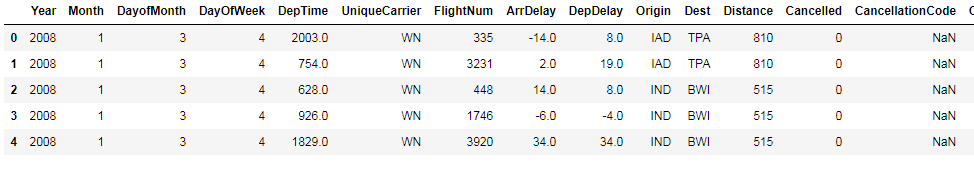
\includegraphics[width=\linewidth,keepaspectratio]{usflights1}
\end{center}
\end{frame}

%%%%%%%%%%%%%%%%%%%%%%%%%%%%%%%%%%%%%%%%%%%%%%%%%%%%%%%%%%
\begin{frame}[fragile]\frametitle{Describe Data}	
Examine data types of all features and total dataframe size in memory.
\begin{lstlisting}
flights_df.info()
>>
<class 'pandas.core.frame.DataFrame'>
RangeIndex: 7009728 entries, 0 to 7009727
Data columns (total 19 columns):
Year                 uint16
Month                uint8
:
NASDelay             float16
SecurityDelay        float16
LateAircraftDelay    float16
dtypes: float16(8), object(4), uint16(3), uint8(4)
memory usage: 387.7+ MB
\end{lstlisting}
\end{frame}

%%%%%%%%%%%%%%%%%%%%%%%%%%%%%%%%%%%%%%%%%%%%%%%%%%%%%%%%%%
\begin{frame}[fragile]\frametitle{Transform Data}	
Change datatypes to standard ones

\begin{lstlisting}
flights_df['Year'] = flights_df['Year'].astype(int)
flights_df['Month'] = flights_df['Month'].astype(int)
flights_df['DayofMonth'] = flights_df['DayofMonth'].astype(int)
flights_df['DayOfWeek'] = flights_df['DayOfWeek'].astype(int)
\end{lstlisting}
\end{frame}

%%%%%%%%%%%%%%%%%%%%%%%%%%%%%%%%%%%%%%%%%%%%%%%%%%%%%%%%%%
\begin{frame}[fragile]\frametitle{Explore Data}	
Count unique Carriers and plot their relative share of flights:
\begin{lstlisting}
flights_df['UniqueCarrier'].nunique()
>> 20

flights_df.groupby('UniqueCarrier').size().plot(kind='bar');
\end{lstlisting}
\begin{center}
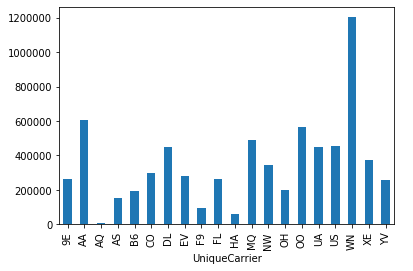
\includegraphics[width=0.6\linewidth,keepaspectratio]{usflights2}
\end{center}
\end{frame}

%%%%%%%%%%%%%%%%%%%%%%%%%%%%%%%%%%%%%%%%%%%%%%%%%%%%%%%%%%
\begin{frame}[fragile]\frametitle{GroupBy}	
We can also group by category/categories in order to calculate different aggregated statistics.

For example, finding top-3 flight codes, that have the largest total distance travelled in year 2008.\begin{lstlisting}
flights_df.groupby(['UniqueCarrier','FlightNum'])['Distance'].sum().sort_values(ascending=False).iloc[:3]

>> 
UniqueCarrier  FlightNum
CO             15           1796244.0
               14           1796244.0
UA             52           1789722.0
Name: Distance, dtype: float64
\end{lstlisting}
\end{frame}

%%%%%%%%%%%%%%%%%%%%%%%%%%%%%%%%%%%%%%%%%%%%%%%%%%%%%%%%%%
\begin{frame}[fragile]\frametitle{GroupBy}	
Another way:
\begin{lstlisting}
flights_df.groupby(['UniqueCarrier','FlightNum'])\
  .agg({'Distance': [np.mean, np.sum, 'count'],
        'Cancelled': np.sum})\
  .sort_values(('Distance', 'sum'), ascending=False)\
  .iloc[0:3]
\end{lstlisting}
\begin{center}
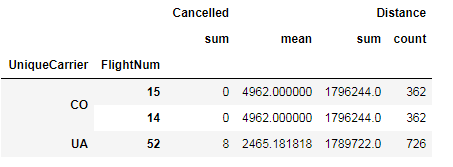
\includegraphics[width=0.6\linewidth,keepaspectratio]{usflights3}
\end{center}
\end{frame}

%%%%%%%%%%%%%%%%%%%%%%%%%%%%%%%%%%%%%%%%%%%%%%%%%%%%%%%%%%
\begin{frame}[fragile]\frametitle{CrossTab}	
Number of flights by days of week and months:
\begin{lstlisting}
pd.crosstab(flights_df.Month, flights_df.DayOfWeek)
\end{lstlisting}
\begin{center}
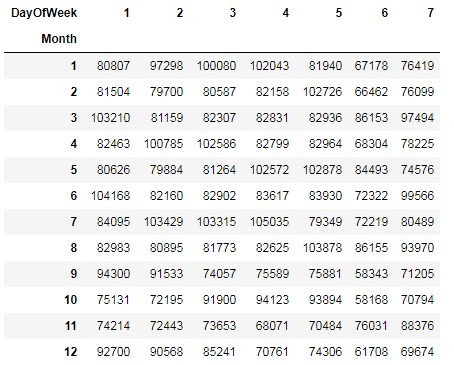
\includegraphics[width=0.6\linewidth,keepaspectratio]{usflights4}
\end{center}
\end{frame}

%%%%%%%%%%%%%%%%%%%%%%%%%%%%%%%%%%%%%%%%%%%%%%%%%%%%%%%%%%
\begin{frame}[fragile]\frametitle{CrossTab}	
It can also be handy to color such tables in order to easily notice outliers:
\begin{lstlisting}
plt.imshow(pd.crosstab(flights_df.Month, flights_df.DayOfWeek),
           cmap='seismic', interpolation='none');
\end{lstlisting}
\begin{center}
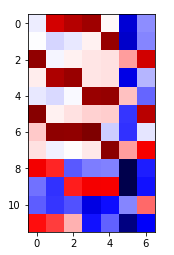
\includegraphics[width=0.3\linewidth,keepaspectratio]{usflights5}
\end{center}
\end{frame}

%%%%%%%%%%%%%%%%%%%%%%%%%%%%%%%%%%%%%%%%%%%%%%%%%%%%%%%%%%
\begin{frame}[fragile]\frametitle{Histogram}	
Flight distance histogram:
\begin{lstlisting}
flights_df.hist('Distance', bins=20);
\end{lstlisting}
\begin{center}
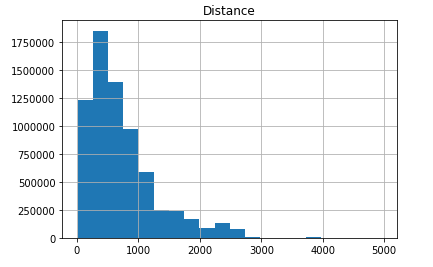
\includegraphics[width=0.5\linewidth,keepaspectratio]{usflights6}
\end{center}
\end{frame}

%%%%%%%%%%%%%%%%%%%%%%%%%%%%%%%%%%%%%%%%%%%%%%%%%%%%%%%%%%
\begin{frame}[fragile]\frametitle{Histogram}	
Making a histogram of flight frequency by date.
\begin{lstlisting}
flights_df['Date'] = pd.to_datetime(flights_df.rename(columns={'DayofMonth': 'Day'})[['Year', 'Month', 'Day']])
num_flights_by_date = flights_df.groupby('Date').size()
num_flights_by_date.plot();
\end{lstlisting}
\begin{center}
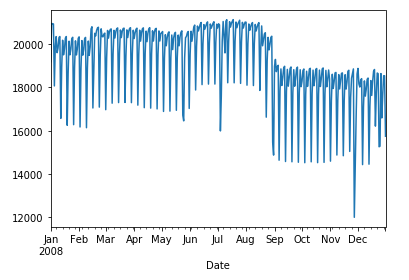
\includegraphics[width=0.5\linewidth,keepaspectratio]{usflights7}
\end{center}
\end{frame}

%%%%%%%%%%%%%%%%%%%%%%%%%%%%%%%%%%%%%%%%%%%%%%%%%%%%%%%%%%
\begin{frame}[fragile]\frametitle{Rolling Window}	
Do you see a weekly pattern above? And below?
\begin{lstlisting}
num_flights_by_date.rolling(window=7).mean().plot();
\end{lstlisting}
\begin{center}
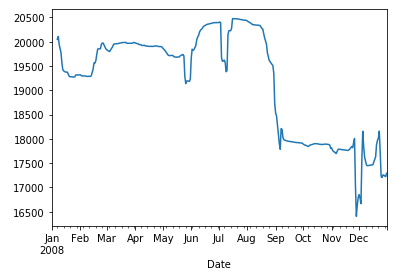
\includegraphics[width=0.5\linewidth,keepaspectratio]{usflights8}
\end{center}
\end{frame}

%%%%%%%%%%%%%%%%%%%%%%%%%%%%%%%%%%%%%%%%%%%%%%%%%%%%%%%%%
\begin{frame}[fragile]\frametitle{Question 1}
Find top-10 carriers in terms of the number of completed flights (UniqueCarrier column)?

Which of the listed below is not in your top-10 list?
\begin{itemize}
\item DL
\item AA
\item OO
\item EV
\end{itemize}

\end{frame}

%%%%%%%%%%%%%%%%%%%%%%%%%%%%%%%%%%%%%%%%%%%%%%%%%%%%%%%%%
\begin{frame}[fragile]\frametitle{Answer 1}
\begin{lstlisting}
flights_df.groupby('UniqueCarrier').size().sort_values(ascending=False).iloc[:10]

>>
UniqueCarrier
WN    1201754
AA     604885
OO     567159
MQ     490693
US     453589
DL     451931
UA     449515
XE     374510
NW     347652
CO     298455
dtype: int64
\end{lstlisting}
Looking at the whole list manually, its, ``EV''
\end{frame}

%%%%%%%%%%%%%%%%%%%%%%%%%%%%%%%%%%%%%%%%%%%%%%%%%%%%%%%%%
\begin{frame}[fragile]\frametitle{Answer 1}
Another way:
\begin{lstlisting}
top10_airlines = flights_df['UniqueCarrier'].value_counts().head(10)
top10_airlines
question_airlines = ['DL','AA', 'OO', 'EV']
set(question_airlines) - set(top10_airlines.index)

>>
{'EV'}
\end{lstlisting}

\end{frame}

%%%%%%%%%%%%%%%%%%%%%%%%%%%%%%%%%%%%%%%%%%%%%%%%%%%%%%%%%
\begin{frame}[fragile]\frametitle{Question 2}
Plot distributions of flight cancellation reasons (CancellationCode).

What is the most frequent reason for flight cancellation? (Use this link to translate codes into reasons)
\begin{itemize}
\item carrier
\item weather conditions
\item National Air System
\item security reasons
\end{itemize}

\end{frame}

%%%%%%%%%%%%%%%%%%%%%%%%%%%%%%%%%%%%%%%%%%%%%%%%%%%%%%%%%
\begin{frame}[fragile]\frametitle{Answer 2}
\begin{lstlisting}
sns.countplot(flights_df['CancellationCode'].sort_values());
\end{lstlisting}
\begin{center}
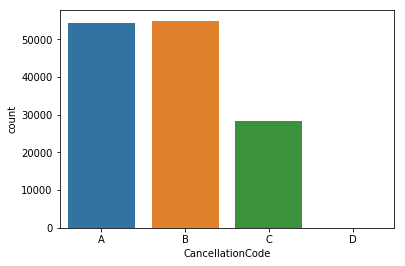
\includegraphics[width=0.6\linewidth,keepaspectratio]{mlcourse1}
\end{center}
\end{frame}

%%%%%%%%%%%%%%%%%%%%%%%%%%%%%%%%%%%%%%%%%%%%%%%%%%%%%%%%%
\begin{frame}[fragile]\frametitle{Answer 2}
\begin{lstlisting}
flights_df['CancellationCode'].mode()
>>
0    B
dtype: object

From the link above:

A - Carrier 
B - Weather 
C - National Air System 
D - Security
\end{lstlisting}

\end{frame}



%%%%%%%%%%%%%%%%%%%%%%%%%%%%%%%%%%%%%%%%%%%%%%%%%%%%%%%%%
\begin{frame}[fragile]\frametitle{Question 3}
Which route is the most frequent, in terms of the number of flights?

(Take a look at 'Origin' and 'Dest' features. Consider $A \rightarrow B$ and $B \rightarrow A$ directions as different routes)
\begin{itemize}
\item New-York – Washington
\item San-Francisco – Los-Angeles
\item San-Jose – Dallas
\item New-York – San-Francisco
\end{itemize}

\end{frame}

%%%%%%%%%%%%%%%%%%%%%%%%%%%%%%%%%%%%%%%%%%%%%%%%%%%%%%%%%
\begin{frame}[fragile]\frametitle{Answer 3}
\begin{lstlisting}
flights_df["Route"] = flights_df["Origin"] + "->" + flights_df["Dest"]
flights_df.groupby('Route').size().sort_values(ascending=False).iloc[:3]
or flights_df['Route'].value_counts().head(3)
>>
Route
SFO-LAX    13788
LAX-SFO    13390
OGG-HNL    12383
dtype: int64
\end{lstlisting}

\end{frame}

%%%%%%%%%%%%%%%%%%%%%%%%%%%%%%%%%%%%%%%%%%%%%%%%%%%%%%%%%
\begin{frame}[fragile]\frametitle{Answer 3}
Or without creating a new feature
\begin{lstlisting}
flights_df[['Origin','Dest']].groupby(['Origin','Dest']).size().idxmax()
>>
('SFO', 'LAX')
\end{lstlisting}

\end{frame}


%%%%%%%%%%%%%%%%%%%%%%%%%%%%%%%%%%%%%%%%%%%%%%%%%%%%%%%%%
\begin{frame}[fragile]\frametitle{Question 4}
Find top-5 delayed routes (count how many times they were delayed on departure). From all flights on these 5 routes, count all flights with weather conditions contributing to a delay.
\begin{itemize}
\item 449
\item 539
\item 549
\item 668
\end{itemize}

\end{frame}

%%%%%%%%%%%%%%%%%%%%%%%%%%%%%%%%%%%%%%%%%%%%%%%%%%%%%%%%%
\begin{frame}[fragile]\frametitle{Answer 4}
Wrong answer!!!
\begin{lstlisting}
top5df = flights_df.groupby(['Route','DepDelay']).size().sort_values(ascending=False).iloc[:5]
a = flights_df[(flights_df["Route"] == "SAN-LAX") & (flights_df["CancellationCode"] == "B")].shape[0]
b = flights_df[(flights_df["Route"] == "LGA-BOS") & (flights_df["CancellationCode"] == "B")].shape[0] 
c = flights_df[(flights_df["Route"] == "DCA-LGA") & (flights_df["CancellationCode"] == "B")].shape[0] 
d = flights_df[(flights_df["Route"] == "LGA-DCA") & (flights_df["CancellationCode"] == "B")].shape[0] 
e = flights_df[(flights_df["Route"] == "BOS-LGA") & (flights_df["CancellationCode"] == "B")].shape[0] 
a+b+c+d+e
>>
Route    DepDelay
SAN-LAX  -5.0        1866
LGA-BOS  -2.0        1854
DCA-LGA  -2.0        1787
LGA-DCA  -2.0        1766
BOS-LGA  -2.0        1720
dtype: int64
639
\end{lstlisting}

\end{frame}

%%%%%%%%%%%%%%%%%%%%%%%%%%%%%%%%%%%%%%%%%%%%%%%%%%%%%%%%%
\begin{frame}[fragile]\frametitle{Answer 4}
Correct answer!!!
\begin{lstlisting}
# find top5 routes with most delayed flights
top5_delayed = flights_df[flights_df['DepDelay'] > 0].groupby('Route').size().sort_values(ascending=False).head(5)
top5_delayed
>>
Route
LAX->SFO    6253
DAL->HOU    5742
SFO->LAX    5322
ORD->LGA    5311
HOU->DAL    5288
dtype: int64
\end{lstlisting}

\end{frame}

%%%%%%%%%%%%%%%%%%%%%%%%%%%%%%%%%%%%%%%%%%%%%%%%%%%%%%%%%
\begin{frame}[fragile]\frametitle{Answer 4}
\begin{lstlisting}
# reduce to only flights from top5 delayed routes
flights_df_top5_delays = flights_df[flights_df['Route'].isin(top5_delayed.index)]
# now the answer
(flights_df_top5_delays['WeatherDelay'] > 0).sum()
>>
668
\end{lstlisting}

\end{frame}

%%%%%%%%%%%%%%%%%%%%%%%%%%%%%%%%%%%%%%%%%%%%%%%%%%%%%%%%%
\begin{frame}[fragile]\frametitle{Question 5}
Examine the hourly distribution of departure times. For that, create a new series from DepTime, removing missing values.

Choose all correct statements:
\begin{itemize}
\item Flights are normally distributed within time interval [0-23] (Search for: Normal distribution, bell curve).
\item Flights are uniformly distributed within time interval [0-23].
\item In the period from 0 am to 4 am there are considerably less flights than from 7 pm to 8 pm.
\end{itemize}

\end{frame}

%%%%%%%%%%%%%%%%%%%%%%%%%%%%%%%%%%%%%%%%%%%%%%%%%%%%%%%%%
\begin{frame}[fragile]\frametitle{Answer 5}
For checking points 1 and 2:
\begin{lstlisting}
dep_hour = (flights_df['DepTime'].dropna() / 100).astype('int') # Only hour portion as int
dep_hour.value_counts(sort=False).plot(kind='bar', 
    title="Number of flights depending on departure hour");
\end{lstlisting}
\begin{center}
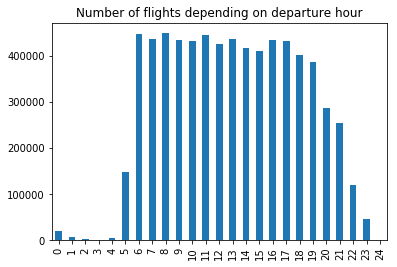
\includegraphics[width=0.6\linewidth,keepaspectratio]{mlcourse2}
\end{center}
\end{frame}

%%%%%%%%%%%%%%%%%%%%%%%%%%%%%%%%%%%%%%%%%%%%%%%%%%%%%%%%%
\begin{frame}[fragile]\frametitle{Answer 5}
For checking point 3:
\begin{lstlisting}
round((dep_hour == 19).sum() / (dep_hour < 5).sum())

>>
12.0
\end{lstlisting}
Correct answers: 3
\end{frame}

%%%%%%%%%%%%%%%%%%%%%%%%%%%%%%%%%%%%%%%%%%%%%%%%%%%%%%%%%
\begin{frame}[fragile]\frametitle{Question 6}
Show how the number of flights changes through time (on the daily/weekly/monthly basis) and interpret the findings.

Choose all correct statements:
\begin{itemize}
\item The number of flights during weekends is less than during weekdays (working days).
\item The lowest number of flights is on Sunday.
\item There are less flights during winter than during summer.
\end{itemize}

\end{frame}

%%%%%%%%%%%%%%%%%%%%%%%%%%%%%%%%%%%%%%%%%%%%%%%%%%%%%%%%%
\begin{frame}[fragile]\frametitle{Answer 6}
\begin{lstlisting}
num_flights_by_day_of_week = flights_df.groupby('DayOfWeek')['FlightNum'].count()
num_flights_by_day_of_week.plot(kind='bar');
\end{lstlisting}
\begin{center}
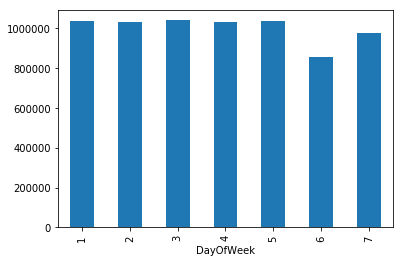
\includegraphics[width=0.6\linewidth,keepaspectratio]{mlcourse3}
\end{center}
\end{frame}

%%%%%%%%%%%%%%%%%%%%%%%%%%%%%%%%%%%%%%%%%%%%%%%%%%%%%%%%%
\begin{frame}[fragile]\frametitle{Answer 6}
\begin{lstlisting}
num_flights_by_month = flights_df.groupby('Month')['FlightNum'].count()
num_flights_by_month.plot(kind='bar');
\end{lstlisting}
\begin{center}
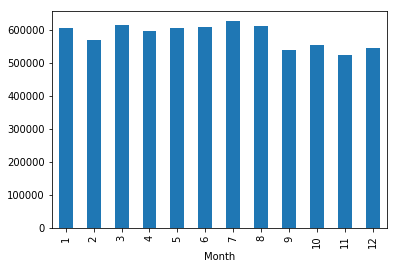
\includegraphics[width=0.6\linewidth,keepaspectratio]{mlcourse4}
\end{center}
Correct answers: 1 and 3
\end{frame}

%%%%%%%%%%%%%%%%%%%%%%%%%%%%%%%%%%%%%%%%%%%%%%%%%%%%%%%%%
\begin{frame}[fragile]\frametitle{Question 7}
Examine the distribution of cancellation reasons with time. Make a bar plot of cancellation reasons aggregated by months.

Choose all correct statements:
\begin{itemize}
\item December has the highest rate of cancellations due to weather.
\item The highest rate of cancellations in September is due to Security reasons.
\item April's top cancellation reason is carriers.
\item Flights cancellations due to National Air System are more frequent than those due to carriers
\end{itemize}

\end{frame}

%%%%%%%%%%%%%%%%%%%%%%%%%%%%%%%%%%%%%%%%%%%%%%%%%%%%%%%%%
\begin{frame}[fragile]\frametitle{Answer 7}
\begin{lstlisting}
# create a month name list
import calendar

month_names = []

for month_idx in flights_df['Month'].unique():
    month_names.append((calendar.month_name[month_idx]))
    
ax = flights_df.groupby(['Month', 'CancellationCode']).size().unstack().plot(kind='bar')

ax.set_xticklabels(month_names, rotation=90)
plt.show()
\end{lstlisting}

\end{frame}

%%%%%%%%%%%%%%%%%%%%%%%%%%%%%%%%%%%%%%%%%%%%%%%%%%%%%%%%%
\begin{frame}[fragile]\frametitle{Answer 7}
\begin{center}
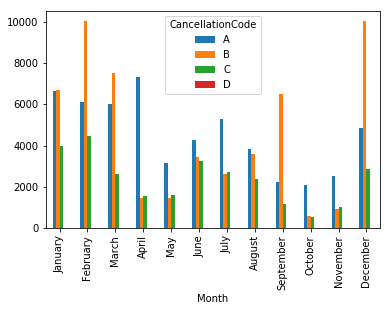
\includegraphics[width=0.6\linewidth,keepaspectratio]{mlcourse5}
\end{center}

\end{frame}


%%%%%%%%%%%%%%%%%%%%%%%%%%%%%%%%%%%%%%%%%%%%%%%%%%%%%%%%%
\begin{frame}[fragile]\frametitle{Question 8}
Which month has the greatest number of cancellations due to Carrier?
\begin{itemize}
\item May
\item January
\item September
\item April
\end{itemize}

\end{frame}

%%%%%%%%%%%%%%%%%%%%%%%%%%%%%%%%%%%%%%%%%%%%%%%%%%%%%%%%%
\begin{frame}[fragile]\frametitle{Answer 8}
\begin{lstlisting}
flights_df.loc[flights_df['CancellationCode'] == 'A', 'Month'].value_counts()
>>
4     7312
1     6635
2     6090
3     6038
7     5292
12    4850
6     4251
8     3852
5     3157
11    2510
9     2246
10    2097
Name: Month, dtype: int64
\end{lstlisting}
April
\end{frame}

%%%%%%%%%%%%%%%%%%%%%%%%%%%%%%%%%%%%%%%%%%%%%%%%%%%%%%%%%
\begin{frame}[fragile]\frametitle{Answer 8}
Or, as a nice plot:
\begin{lstlisting}
import matplotlib.colors as colors
import random 
import calendar

ax = flights_df[flights_df['CancellationCode'] == 'A']\
                                        .groupby(['Month'])['UniqueCarrier']\
                                        .count().plot(kind='bar', color='coral')
ax.set_xticklabels(month_names, rotation=90)
plt.show()
\end{lstlisting}
\begin{center}
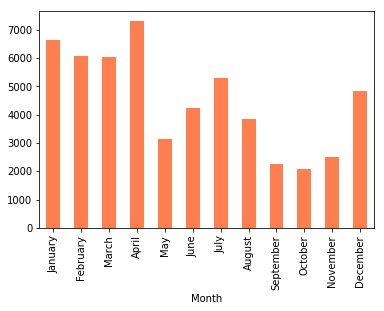
\includegraphics[width=0.35\linewidth,keepaspectratio]{mlcourse6}
\end{center}
\end{frame}
%%%%%%%%%%%%%%%%%%%%%%%%%%%%%%%%%%%%%%%%%%%%%%%%%%%%%%%%%
\begin{frame}[fragile]\frametitle{Question 9}
 Identify the carrier with the greatest number of cancellations due to carrier in the corresponding month from the previous question.
 \begin{itemize}
\item 9E
\item EV
\item HA
\item AA
\end{itemize}

\end{frame}

%%%%%%%%%%%%%%%%%%%%%%%%%%%%%%%%%%%%%%%%%%%%%%%%%%%%%%%%%
\begin{frame}[fragile]\frametitle{Answer 9}
\begin{lstlisting}
flights_df.loc[(flights_df['CancellationCode'] == 'A') & (flights_df['Month'] == 4),
               'UniqueCarrier'].value_counts().head()
			   
>>
AA    3696
WN     533
UA     494
YV     454
9E     391
Name: UniqueCarrier, dtype: int64			   
\end{lstlisting}
AA
\end{frame}


%%%%%%%%%%%%%%%%%%%%%%%%%%%%%%%%%%%%%%%%%%%%%%%%%%%%%%%%%
\begin{frame}[fragile]\frametitle{Question 10}
Examine median arrival and departure delays (in time) by carrier. Which carrier has the lowest median delay time for both arrivals and departures? Leave only non-negative values of delay times ('ArrDelay', 'DepDelay'). Boxplots can be helpful in this exercise, as well as it might be a good idea to remove outliers in order to build nice graphs. You can exclude delay time values higher than a corresponding .95 percentile.
 \begin{itemize}
\item EV
\item OO
\item AA
\item AQ
\end{itemize}

\end{frame}

%%%%%%%%%%%%%%%%%%%%%%%%%%%%%%%%%%%%%%%%%%%%%%%%%%%%%%%%%
\begin{frame}[fragile]\frametitle{Answer 10}
\begin{lstlisting}
for delay_type in ['ArrDelay', 'DepDelay']:
    sub_df = flights_df[(flights_df[delay_type] >= 0) &
                        (flights_df[delay_type] < flights_df[delay_type].quantile(.95))]
    sns.boxplot(x='UniqueCarrier', y=delay_type, data=sub_df);
    plt.show()
\end{lstlisting}
\begin{center}
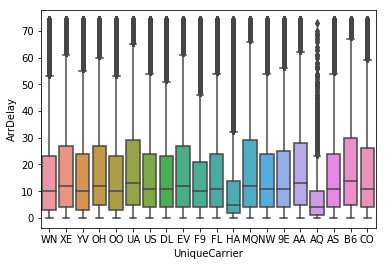
\includegraphics[width=0.35\linewidth,keepaspectratio]{mlcourse7}
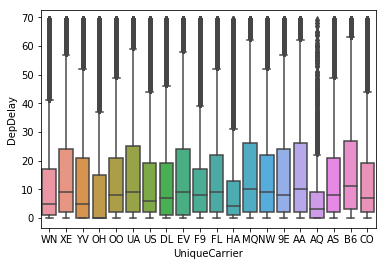
\includegraphics[width=0.35\linewidth,keepaspectratio]{mlcourse8}

\end{center}
AQ
\end{frame}